% Created by tikzDevice version 0.12 on 2019-03-27 17:35:08
% !TEX encoding = UTF-8 Unicode
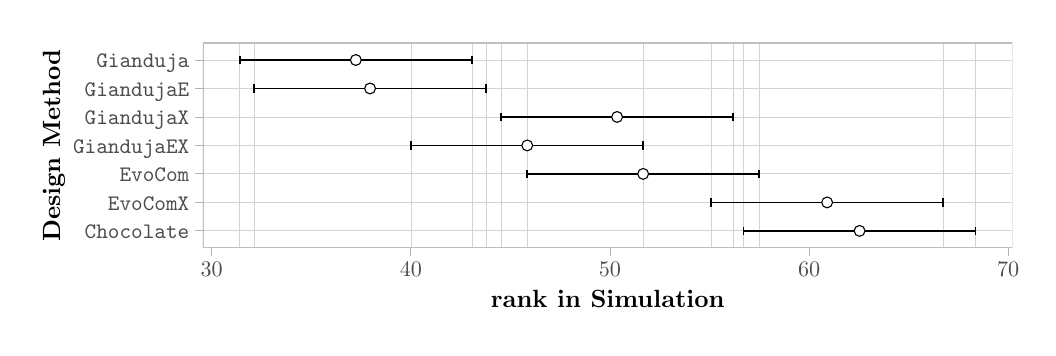
\begin{tikzpicture}[x=1pt,y=1pt]
\definecolor{fillColor}{RGB}{255,255,255}
\path[use as bounding box,fill=fillColor,fill opacity=0.00] (0,0) rectangle (361.35,108.41);
\begin{scope}
\path[clip] (  0.00,  0.00) rectangle (361.35,108.40);
\definecolor{drawColor}{RGB}{255,255,255}
\definecolor{fillColor}{RGB}{255,255,255}

\path[draw=drawColor,line width= 0.6pt,line join=round,line cap=round,fill=fillColor] (  0.00,  0.00) rectangle (361.35,108.40);
\end{scope}
\begin{scope}
\path[clip] ( 63.34, 28.81) rectangle (355.85,102.90);
\definecolor{fillColor}{RGB}{255,255,255}

\path[fill=fillColor] ( 63.34, 28.81) rectangle (355.85,102.90);
\definecolor{drawColor}{RGB}{211,211,211}

\path[draw=drawColor,line width= 0.3pt,line join=round] ( 63.34, 55.57) --
	(355.85, 55.57);

\path[draw=drawColor,line width= 0.3pt,line join=round] ( 63.34, 45.27) --
	(355.85, 45.27);

\path[draw=drawColor,line width= 0.3pt,line join=round] ( 63.34, 96.73) --
	(355.85, 96.73);

\path[draw=drawColor,line width= 0.3pt,line join=round] ( 63.34, 86.44) --
	(355.85, 86.44);

\path[draw=drawColor,line width= 0.3pt,line join=round] ( 63.34, 76.15) --
	(355.85, 76.15);

\path[draw=drawColor,line width= 0.3pt,line join=round] ( 63.34, 65.86) --
	(355.85, 65.86);

\path[draw=drawColor,line width= 0.3pt,line join=round] ( 63.34, 34.98) --
	(355.85, 34.98);

\path[draw=drawColor,line width= 0.2pt,line join=round] (342.55, 28.81) -- (342.55,102.90);

\path[draw=drawColor,line width= 0.2pt,line join=round] (264.35, 28.81) -- (264.35,102.90);

\path[draw=drawColor,line width= 0.2pt,line join=round] (330.82, 28.81) -- (330.82,102.90);

\path[draw=drawColor,line width= 0.2pt,line join=round] (160.53, 28.81) -- (160.53,102.90);

\path[draw=drawColor,line width= 0.2pt,line join=round] (165.67, 28.81) -- (165.67,102.90);

\path[draw=drawColor,line width= 0.2pt,line join=round] (222.46, 28.81) -- (222.46,102.90);

\path[draw=drawColor,line width= 0.2pt,line join=round] (254.92, 28.81) -- (254.92,102.90);

\path[draw=drawColor,line width= 0.2pt,line join=round] (258.67, 28.81) -- (258.67,102.90);

\path[draw=drawColor,line width= 0.2pt,line join=round] (180.46, 28.81) -- (180.46,102.90);

\path[draw=drawColor,line width= 0.2pt,line join=round] (246.93, 28.81) -- (246.93,102.90);

\path[draw=drawColor,line width= 0.2pt,line join=round] ( 76.64, 28.81) -- ( 76.64,102.90);

\path[draw=drawColor,line width= 0.2pt,line join=round] ( 81.78, 28.81) -- ( 81.78,102.90);

\path[draw=drawColor,line width= 0.2pt,line join=round] (138.57, 28.81) -- (138.57,102.90);

\path[draw=drawColor,line width= 0.2pt,line join=round] (171.04, 28.81) -- (171.04,102.90);
\definecolor{drawColor}{RGB}{0,0,0}

\path[draw=drawColor,line width= 0.6pt,line join=round] (342.55, 33.44) --
	(342.55, 36.53);

\path[draw=drawColor,line width= 0.6pt,line join=round] (342.55, 34.98) --
	(258.67, 34.98);

\path[draw=drawColor,line width= 0.6pt,line join=round] (258.67, 33.44) --
	(258.67, 36.53);

\path[draw=drawColor,line width= 0.6pt,line join=round] (264.35, 54.02) --
	(264.35, 57.11);

\path[draw=drawColor,line width= 0.6pt,line join=round] (264.35, 55.57) --
	(180.46, 55.57);

\path[draw=drawColor,line width= 0.6pt,line join=round] (180.46, 54.02) --
	(180.46, 57.11);

\path[draw=drawColor,line width= 0.6pt,line join=round] (330.82, 43.73) --
	(330.82, 46.82);

\path[draw=drawColor,line width= 0.6pt,line join=round] (330.82, 45.27) --
	(246.93, 45.27);

\path[draw=drawColor,line width= 0.6pt,line join=round] (246.93, 43.73) --
	(246.93, 46.82);

\path[draw=drawColor,line width= 0.6pt,line join=round] (160.53, 95.19) --
	(160.53, 98.27);

\path[draw=drawColor,line width= 0.6pt,line join=round] (160.53, 96.73) --
	( 76.64, 96.73);

\path[draw=drawColor,line width= 0.6pt,line join=round] ( 76.64, 95.19) --
	( 76.64, 98.27);

\path[draw=drawColor,line width= 0.6pt,line join=round] (165.67, 84.90) --
	(165.67, 87.98);

\path[draw=drawColor,line width= 0.6pt,line join=round] (165.67, 86.44) --
	( 81.78, 86.44);

\path[draw=drawColor,line width= 0.6pt,line join=round] ( 81.78, 84.90) --
	( 81.78, 87.98);

\path[draw=drawColor,line width= 0.6pt,line join=round] (222.46, 64.31) --
	(222.46, 67.40);

\path[draw=drawColor,line width= 0.6pt,line join=round] (222.46, 65.86) --
	(138.57, 65.86);

\path[draw=drawColor,line width= 0.6pt,line join=round] (138.57, 64.31) --
	(138.57, 67.40);

\path[draw=drawColor,line width= 0.6pt,line join=round] (254.92, 74.60) --
	(254.92, 77.69);

\path[draw=drawColor,line width= 0.6pt,line join=round] (254.92, 76.15) --
	(171.04, 76.15);

\path[draw=drawColor,line width= 0.6pt,line join=round] (171.04, 74.60) --
	(171.04, 77.69);

\path[draw=drawColor,line width= 0.4pt,line join=round,line cap=round,fill=fillColor] (300.61, 34.98) circle (  1.96);

\path[draw=drawColor,line width= 0.4pt,line join=round,line cap=round,fill=fillColor] (222.40, 55.57) circle (  1.96);

\path[draw=drawColor,line width= 0.4pt,line join=round,line cap=round,fill=fillColor] (288.88, 45.27) circle (  1.96);

\path[draw=drawColor,line width= 0.4pt,line join=round,line cap=round,fill=fillColor] (118.58, 96.73) circle (  1.96);

\path[draw=drawColor,line width= 0.4pt,line join=round,line cap=round,fill=fillColor] (123.72, 86.44) circle (  1.96);

\path[draw=drawColor,line width= 0.4pt,line join=round,line cap=round,fill=fillColor] (180.52, 65.86) circle (  1.96);

\path[draw=drawColor,line width= 0.4pt,line join=round,line cap=round,fill=fillColor] (212.98, 76.15) circle (  1.96);
\definecolor{drawColor}{RGB}{190,190,190}

\path[draw=drawColor,line width= 0.6pt,line join=round,line cap=round] ( 63.34, 28.81) rectangle (355.85,102.90);
\end{scope}
\begin{scope}
\path[clip] (  0.00,  0.00) rectangle (361.35,108.41);
\definecolor{drawColor}{gray}{0.30}

\node[text=drawColor,anchor=base east,inner sep=0pt, outer sep=0pt, scale=  0.80] at ( 58.39, 52.81) {\texttt{EvoCom}};

\node[text=drawColor,anchor=base east,inner sep=0pt, outer sep=0pt, scale=  0.80] at ( 58.39, 42.52) {\texttt{EvoComX}};

\node[text=drawColor,anchor=base east,inner sep=0pt, outer sep=0pt, scale=  0.80] at ( 58.39, 93.98) {\texttt{Gianduja}};

\node[text=drawColor,anchor=base east,inner sep=0pt, outer sep=0pt, scale=  0.80] at ( 58.39, 83.68) {\texttt{GiandujaE}};

\node[text=drawColor,anchor=base east,inner sep=0pt, outer sep=0pt, scale=  0.80] at ( 58.39, 73.39) {\texttt{GiandujaX}};

\node[text=drawColor,anchor=base east,inner sep=0pt, outer sep=0pt, scale=  0.80] at ( 58.39, 63.10) {\texttt{GiandujaEX}};

\node[text=drawColor,anchor=base east,inner sep=0pt, outer sep=0pt, scale=  0.80] at ( 58.39, 32.23) {\texttt{Chocolate}};
\end{scope}
\begin{scope}
\path[clip] (  0.00,  0.00) rectangle (361.35,108.41);
\definecolor{drawColor}{gray}{0.70}

\path[draw=drawColor,line width= 0.3pt,line join=round] ( 60.59, 55.57) --
	( 63.34, 55.57);

\path[draw=drawColor,line width= 0.3pt,line join=round] ( 60.59, 45.27) --
	( 63.34, 45.27);

\path[draw=drawColor,line width= 0.3pt,line join=round] ( 60.59, 96.73) --
	( 63.34, 96.73);

\path[draw=drawColor,line width= 0.3pt,line join=round] ( 60.59, 86.44) --
	( 63.34, 86.44);

\path[draw=drawColor,line width= 0.3pt,line join=round] ( 60.59, 76.15) --
	( 63.34, 76.15);

\path[draw=drawColor,line width= 0.3pt,line join=round] ( 60.59, 65.86) --
	( 63.34, 65.86);

\path[draw=drawColor,line width= 0.3pt,line join=round] ( 60.59, 34.98) --
	( 63.34, 34.98);
\end{scope}
\begin{scope}
\path[clip] (  0.00,  0.00) rectangle (361.35,108.41);
\definecolor{drawColor}{gray}{0.70}

\path[draw=drawColor,line width= 0.3pt,line join=round] ( 66.50, 26.06) --
	( 66.50, 28.81);

\path[draw=drawColor,line width= 0.3pt,line join=round] (138.46, 26.06) --
	(138.46, 28.81);

\path[draw=drawColor,line width= 0.3pt,line join=round] (210.41, 26.06) --
	(210.41, 28.81);

\path[draw=drawColor,line width= 0.3pt,line join=round] (282.37, 26.06) --
	(282.37, 28.81);

\path[draw=drawColor,line width= 0.3pt,line join=round] (354.32, 26.06) --
	(354.32, 28.81);
\end{scope}
\begin{scope}
\path[clip] (  0.00,  0.00) rectangle (361.35,108.41);
\definecolor{drawColor}{gray}{0.30}

\node[text=drawColor,anchor=base,inner sep=0pt, outer sep=0pt, scale=  0.80] at ( 66.50, 18.35) {30};

\node[text=drawColor,anchor=base,inner sep=0pt, outer sep=0pt, scale=  0.80] at (138.46, 18.35) {40};

\node[text=drawColor,anchor=base,inner sep=0pt, outer sep=0pt, scale=  0.80] at (210.41, 18.35) {50};

\node[text=drawColor,anchor=base,inner sep=0pt, outer sep=0pt, scale=  0.80] at (282.37, 18.35) {60};

\node[text=drawColor,anchor=base,inner sep=0pt, outer sep=0pt, scale=  0.80] at (354.32, 18.35) {70};
\end{scope}
\begin{scope}
\path[clip] (  0.00,  0.00) rectangle (361.35,108.41);
\definecolor{drawColor}{RGB}{0,0,0}

\node[text=drawColor,anchor=base,inner sep=0pt, outer sep=0pt, scale=  0.90] at (209.60,  7.44) {\bfseries rank in Simulation};
\end{scope}
\begin{scope}
\path[clip] (  0.00,  0.00) rectangle (361.35,108.41);
\definecolor{drawColor}{RGB}{0,0,0}

\node[text=drawColor,rotate= 90.00,anchor=base,inner sep=0pt, outer sep=0pt, scale=  0.90] at ( 11.71, 65.86) {\bfseries Design Method};
\end{scope}
\end{tikzpicture}
